\section{Fanny Shafira Damayanti (1174069)}
\subsection{Instalasi Map Server}
\begin{enumerate}
    \item Langkah pertama yaitu mendownload terlebih dahulu map servernya, untuk download Map Server bisa kunjungi seperti gambar di bawah ini.
  \hfill\break
  \begin{figure}[H]
  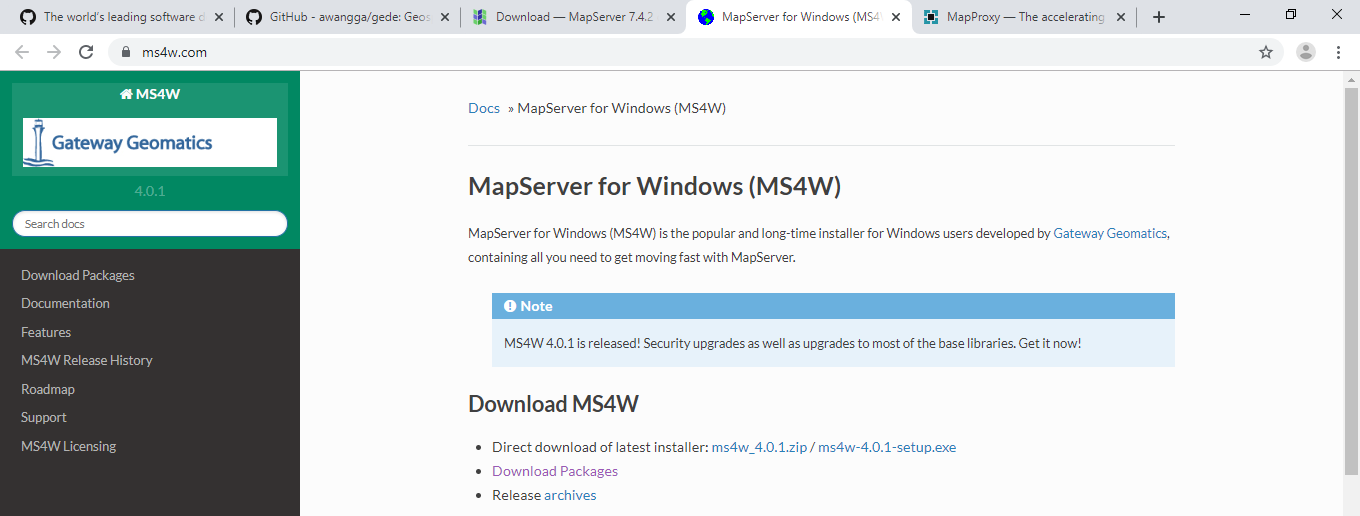
\includegraphics[width=4cm]{figures/tugas4/1174069/1.png}
  \centering
  \caption{Download File MS4W}
  \end{figure}
    
   

    \item Setelah di download, kita akan lakukan proses Instalasi. Untuk versi windows bisa saya sarankan mendownload yang .exe agar lebih mudah saat instalasi.
   
    
  \hfill\break
  \begin{figure}[H]
  
\includegraphics[width=4cm]{figures/tugas4/1174069/2.png}
  \centering
  \caption{Install File exe}
  \end{figure}
    
    

\end{enumerate}


\subsection{Konfigurasi Map Server}
Setelah proses instalasi nya selesai, proses selanjutnya yaitu konfigurasi. 
\begin{enumerate}
  \item Buka folder ms4w. Masuk ke folder apache
  
\hfill\break
  \begin{figure}[H]
  
\includegraphics[width=4cm]{figures/tugas4/1174069/3.png}
  \centering
  \caption{Isi Folder apache}
  \end{figure}

  \item Masuk ke folder conf
	
	\hfill\break
  \begin{figure}[H]
  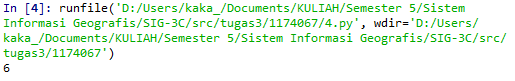
\includegraphics[width=4cm]{figures/tugas4/1174069/4.png}
  \centering
  \caption{Isi Folder conf}
  \end{figure}
  
  \item Buka file httpd.conf dan ubah listen port nya menjadi port 80.
  
\hfill\break
  \begin{figure}[H]
  
\includegraphics[width=4cm]{figures/tugas4/1174069/5.png}
  \centering
  \caption{Listen port 80}
  \end{figure}
  
  \item Kemudian kita jalankan servisnya, dengan menggunakan tombol windows + r dan ketikan services.msc
    
  \hfill\break
  \begin{figure}[H]
  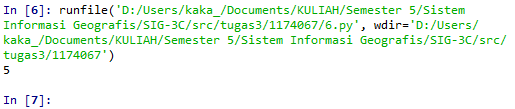
\includegraphics[width=4cm]{figures/tugas4/1174069/6.png}
  \centering
  \caption{Mengakses Halaman Service}
  \end{figure}
  

  \item Cari servis untuk Apache MS4W Web Server
    
    \hfill\break
  \begin{figure}[H]
  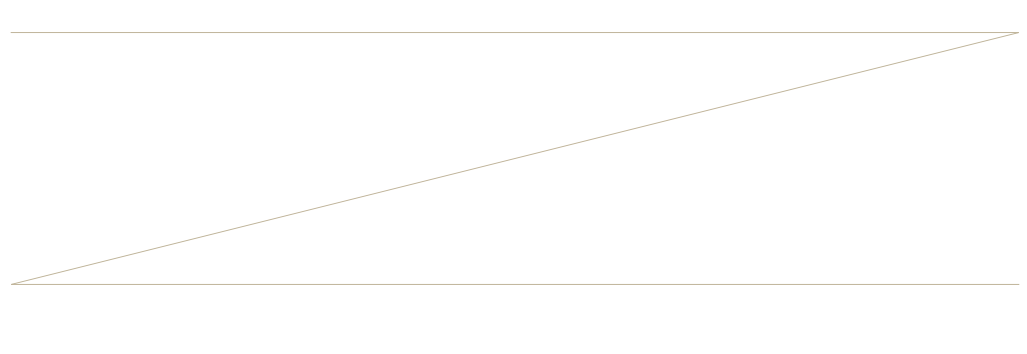
\includegraphics[width=4cm]{figures/tugas4/1174069/7.png}
  \centering
  \caption{Pengaturan Service Apache MS4W Web Server}
  \end{figure}

  \item Jika sudah menemukannya klik 2x
  \item Dan setting seperti berikut
 
    
    \hfill\break
  \begin{figure}[H]
  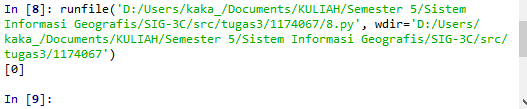
\includegraphics[width=4cm]{figures/tugas4/1174069/8.png}
  \centering
  \caption{Pengaturan Service Apache MS4W Web Server}
  \end{figure}

\end{enumerate}


\subsection{Pengujian}
\begin{enumerate}
  \item Download atau clone file di https://github.com/awangga/gede


 \hfill\break
  \begin{figure}[H]
  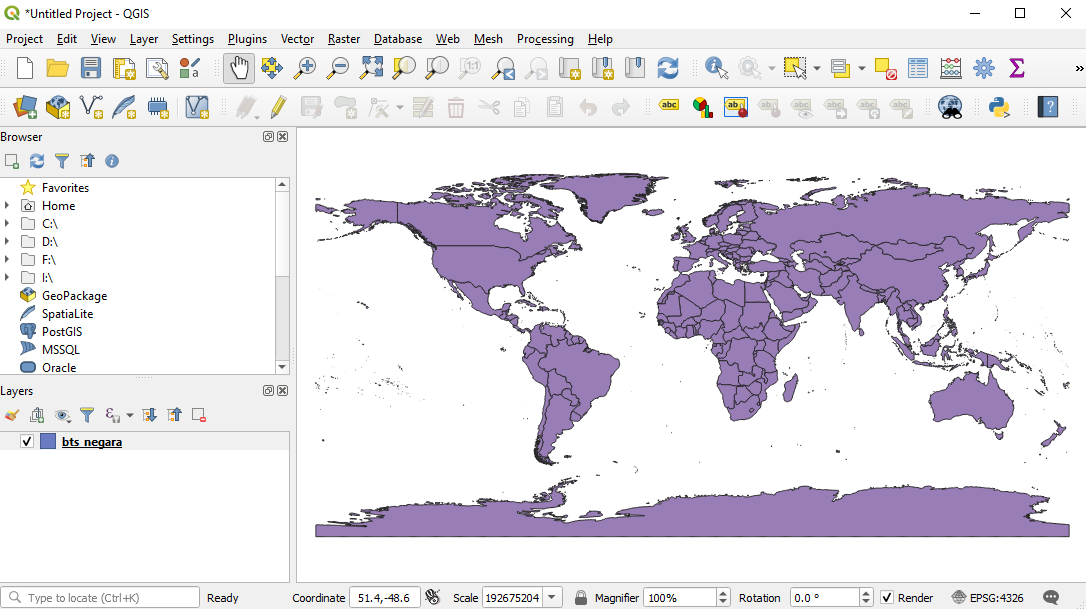
\includegraphics[width=4cm]{figures/tugas4/1174069/9.png}
  \centering
  \caption{Download atau clone file di github}
  \end{figure}


  \item masuk ke folder shp
  
    \hfill\break
    \begin{figure}[H]
  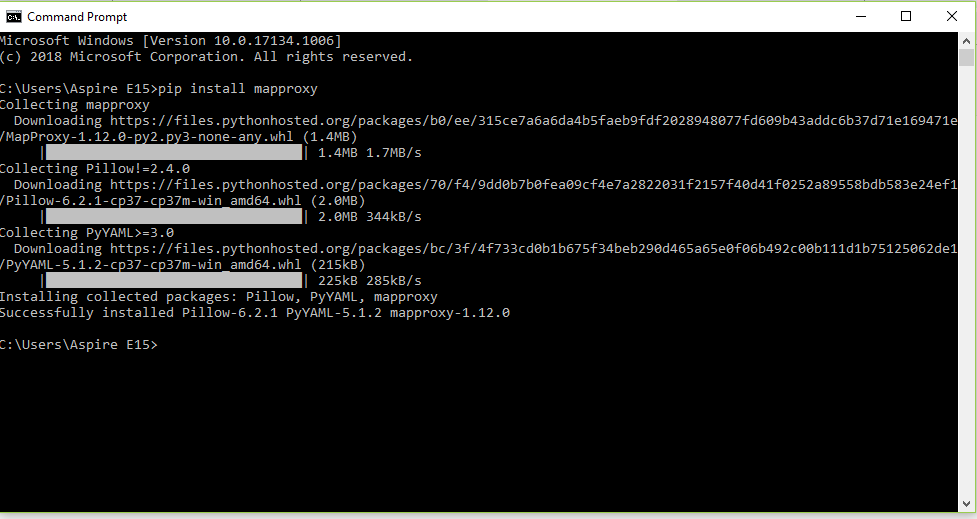
\includegraphics[width=4cm]{figures/tugas4/1174069/10.png}
  \centering
  \caption{Isi folder shp}
  \end{figure}

  \item jalankan file 00.shp di aplikasi QGIS
    
    \hfill\break
    \begin{figure}[H]
  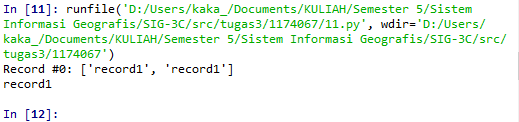
\includegraphics[width=4cm]{figures/tugas4/1174069/11.png}
  \centering
  \caption{Hasil Gambar file 00}
  \end{figure}

  \item Selajutnya jalankan file btsnegara
  
 \hfill\break
    \begin{figure}[H]
  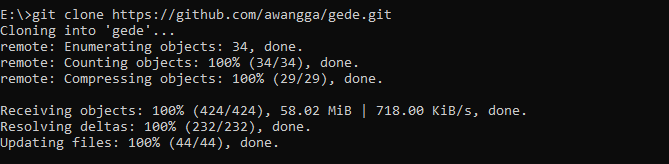
\includegraphics[width=4cm]{figures/tugas4/1174069/12.png}
  \centering
  \caption{Hasil Gambar file btsnegara}
  \end{figure}
 
\end{enumerate}
\subsection{Link Youtube Instalasi MapServer}
{https://youtu.be/wp1E2JovMcA}

\subsection{Instalasi MapProxy}
\begin{enumerate}
  \item Langkah pertama buka Command Prompt
  \item Lalu ketikkan pip install MapProxy
  \hfill\break
  \begin{figure}[H]
  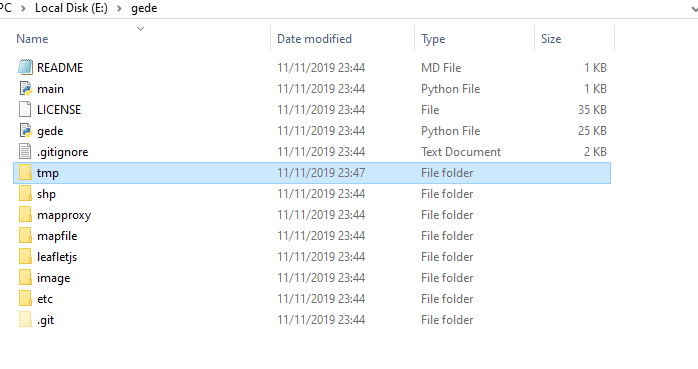
\includegraphics[width=4cm]{figures/tugas4/1174069/13.png}
  \centering
  \caption{Instalasi MapProxy}
  \end{figure}
  
  \item Selanjutnya ketikkan pip install PyProj
  \hfill\break
  \begin{figure}[H]
  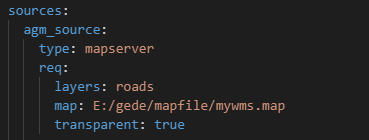
\includegraphics[width=4cm]{figures/tugas4/1174069/14.png}
  \centering
  \caption{Instalasi PyProj}
  \end{figure}
\end{enumerate}

\subsection{Membuka map menggunakan MapProxy}
\begin{enumerate}
  \item Langkah pertama kita akan mendownload / clone git dari https://github.com/awangga/gede
  \item Pastikan path menuju folder gede tidak ada spasi contohnya saya F:/gede-master
  \item Pada folder gede-master buat folder bernama tmp
  \hfill\break
  \begin{figure}[H]
  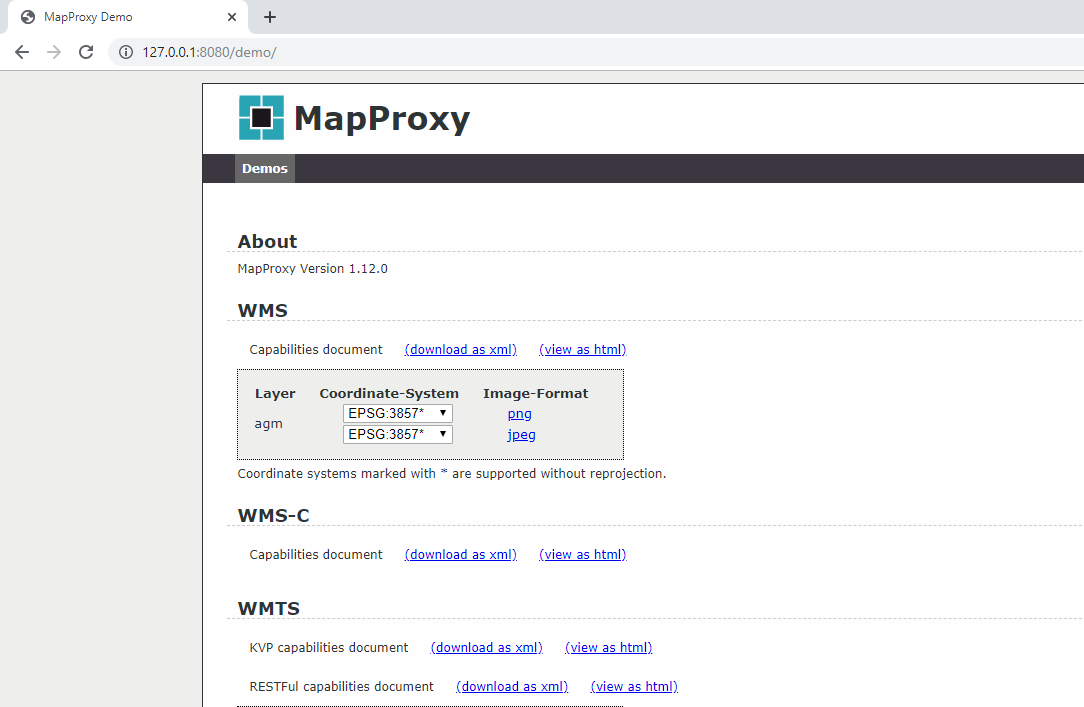
\includegraphics[width=4cm]{figures/tugas4/1174069/15.png}
  \centering
  \caption{Membuat folder baru tmp}
  \end{figure}

  \item Kemudian buka folder mapproxy lalu edit file agm.yaml
  \hfill\break
  \begin{figure}[H]
  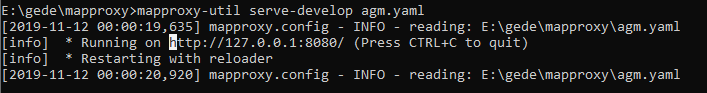
\includegraphics[width=4cm]{figures/tugas4/1174069/16.png}
  \centering
  \caption{File agm.yaml}
  \end{figure}

  \item Edit pada bagian sources lalu ada map, masukkan pathnya sesuai dengan dimana kita menyimpan file gede. Di laptop saya, saya menyimpan nya di F:/gede-master/mapfile/mywms.map
  \hfill\break
  \begin{figure}[H]
  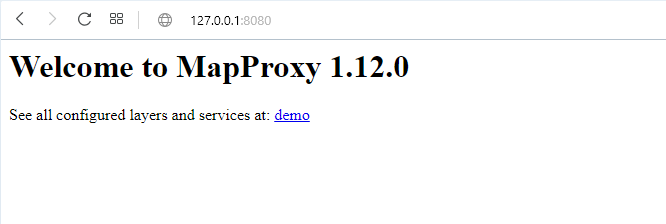
\includegraphics[width=4cm]{figures/tugas4/1174069/17.png}
  \centering
  \caption{Edit lokasi mywms.map}
  \end{figure}


  \item Setelah itu dibawahnya pada bagian binary masukkan lokasi instalasi ms4wnya, lalu tambahkan /Apache/cgi-bin/mapserv.exe, setelah diedit menjadi C:/ms4w/Apache/cgi-bin/mapserv.exe
  \hfill\break
  \begin{figure}[H]
  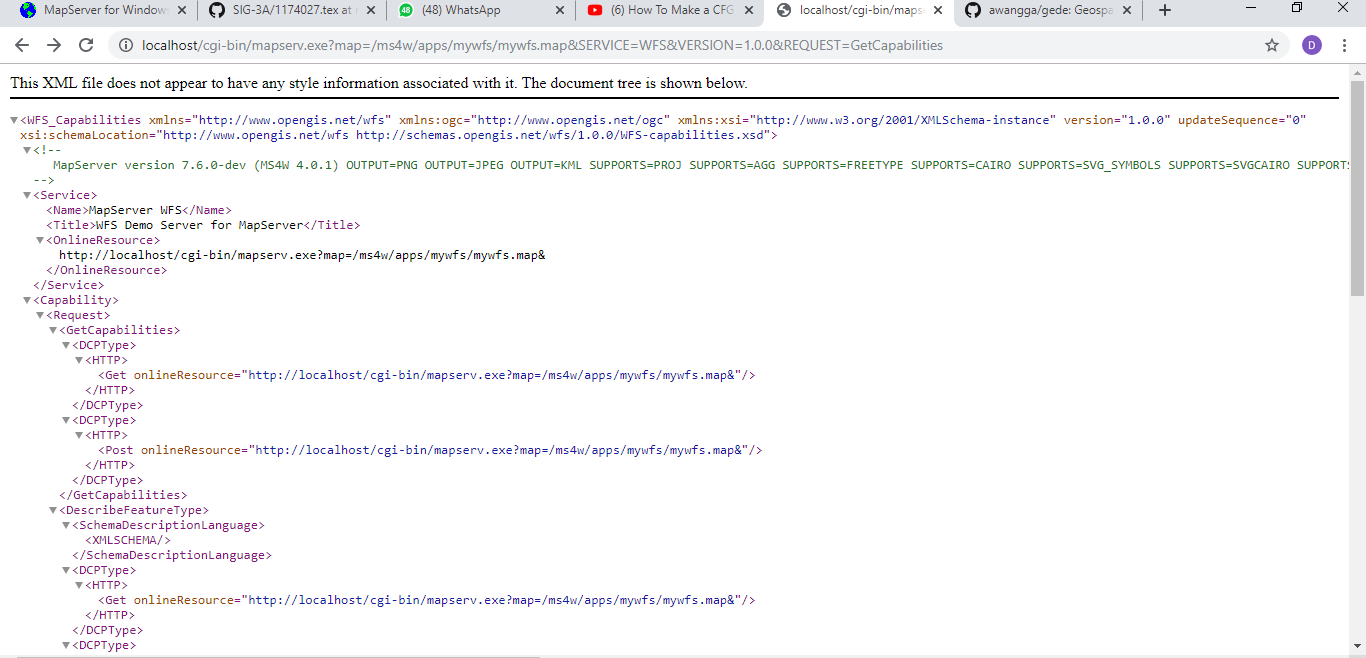
\includegraphics[width=4cm]{figures/tugas4/1174069/18.png}
  \centering
  \caption{Edit path binary mapserv}
  \end{figure}

  \item Kemudian pada bagian working-dir masukkan path folder yang telah dibuat sebelumnya, yaitu F:/gede-master/tmp
  \hfill\break
  \begin{figure}[H]
  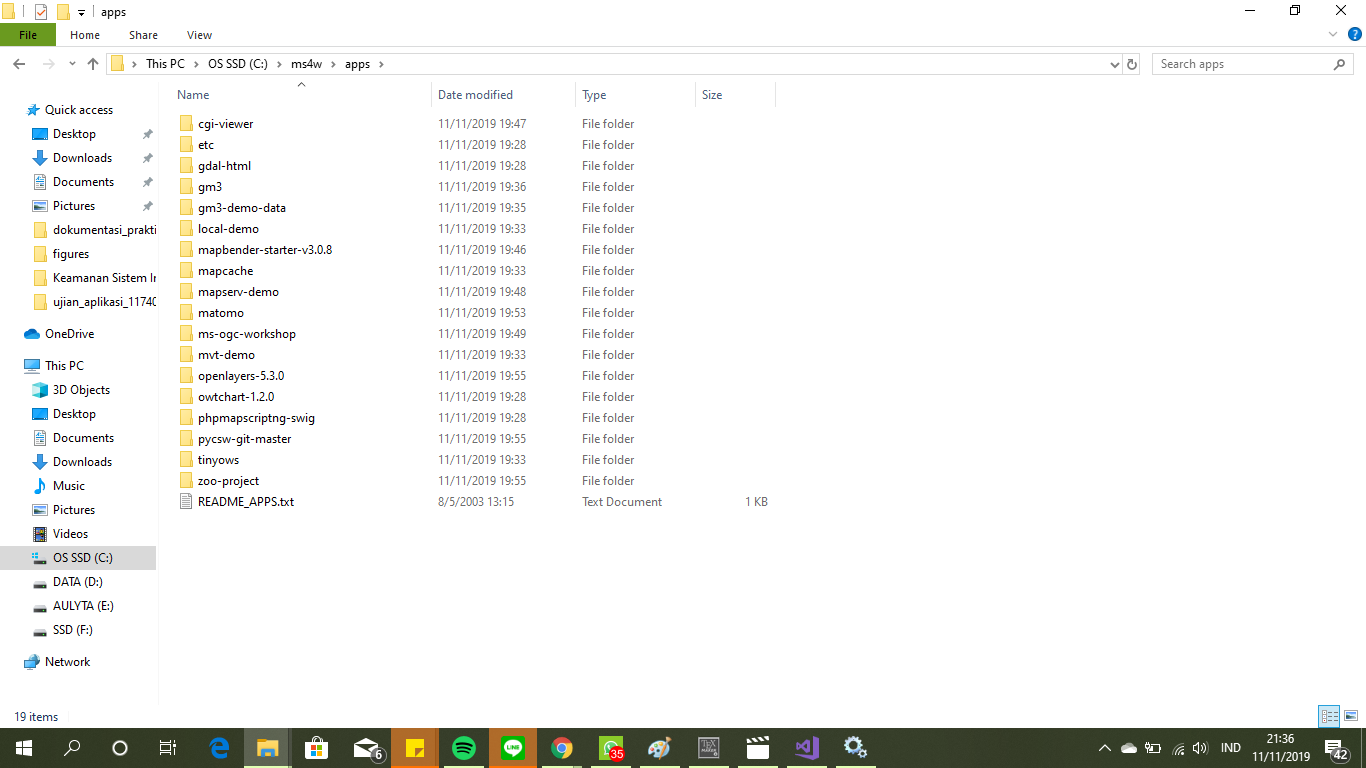
\includegraphics[width=4cm]{figures/tugas4/1174069/19.png}
  \centering
  \caption{Edit path working-dir}
  \end{figure}

  \item Selanjutnya buka aplikasi MS4W-Shell
  \hfill\break
  \begin{figure}[H]
  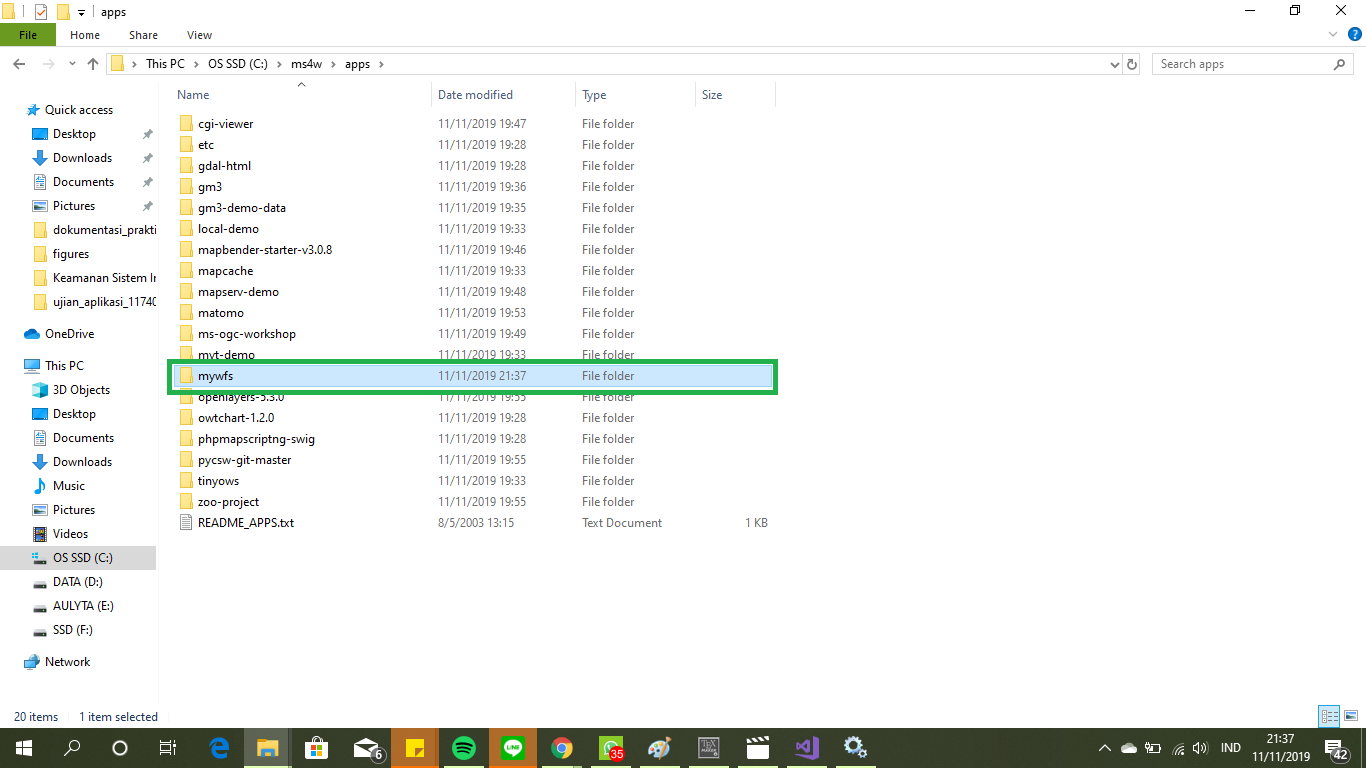
\includegraphics[width=4cm]{figures/tugas4/1174069/20.png}
  \centering
  \caption{Aplikasi MS4W-Shell}
  \end{figure}

  \item Setelah itu buka lokasi folder gede kita yang tadi telah di clone
  \hfill\break
  \begin{figure}[H]
  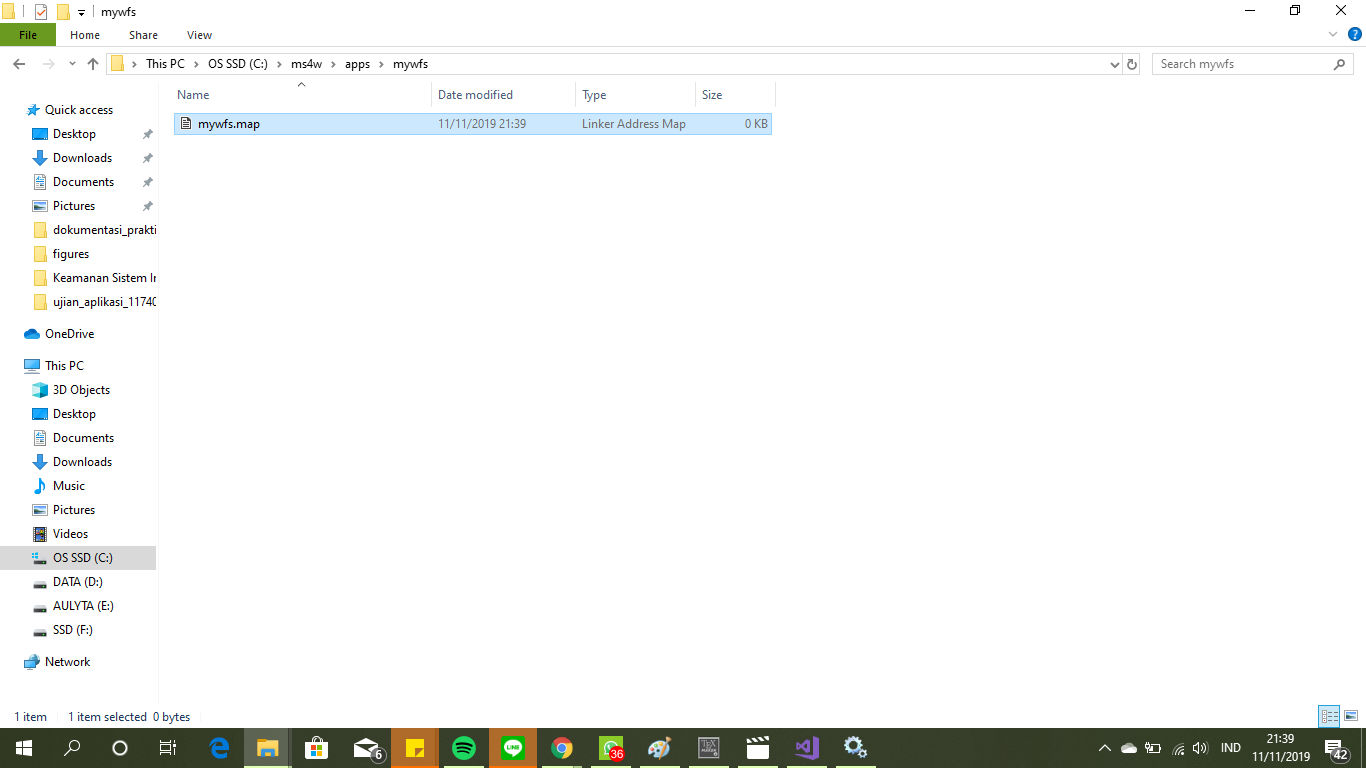
\includegraphics[width=4cm]{figures/tugas4/1174069/21.png}
  \centering
  \caption{Buka Folder gede}
  \end{figure}

  \item Setelah itu buka folder mapproxy yang ada pada folder gede
  \hfill\break
  \begin{figure}[H]
  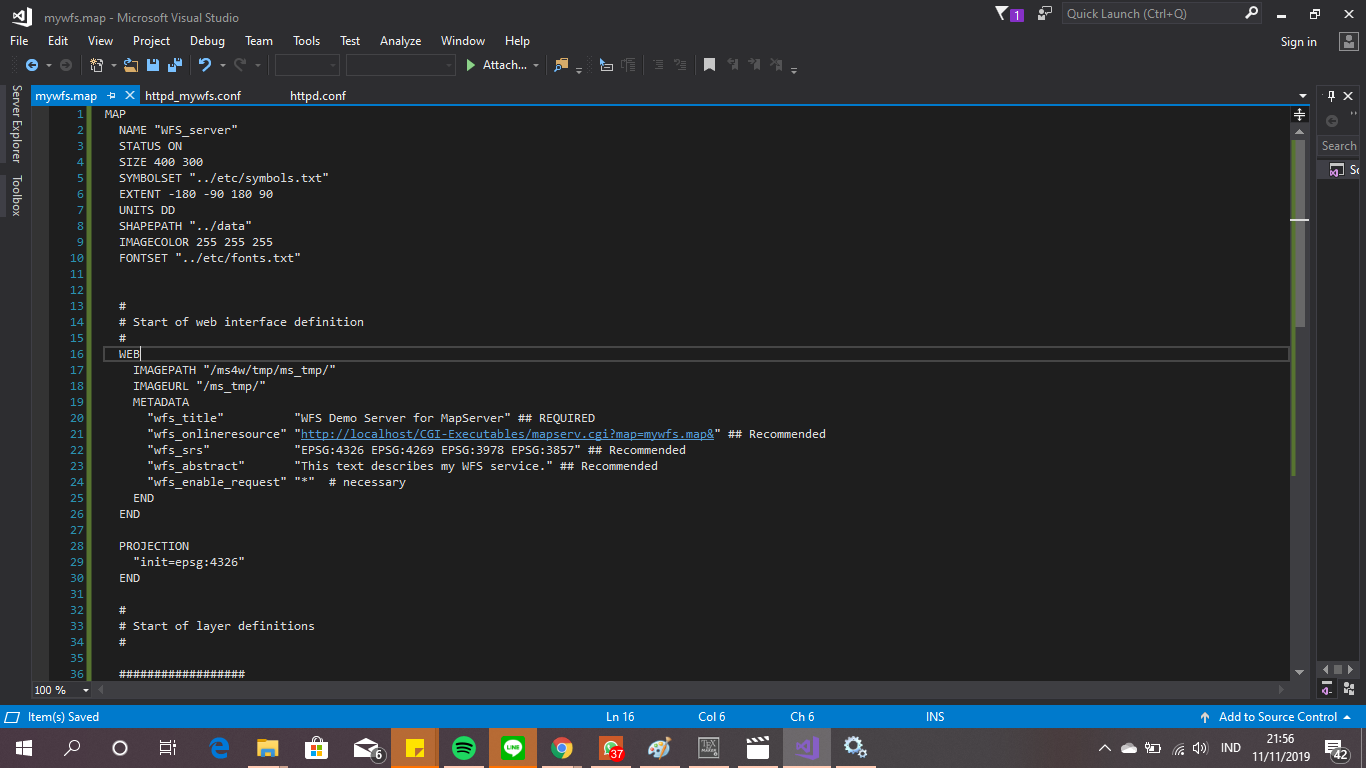
\includegraphics[width=4cm]{figures/tugas4/1174069/22.png}
  \centering
  \caption{Buka Folder mapproxy}
  \end{figure}

  \item ketikkan "mapproxy-util serve-develop ./agm.yaml" pada ms4w-Shell untuk membuka aplikasi mapproxy
  \hfill\break
  \begin{figure}[H]
  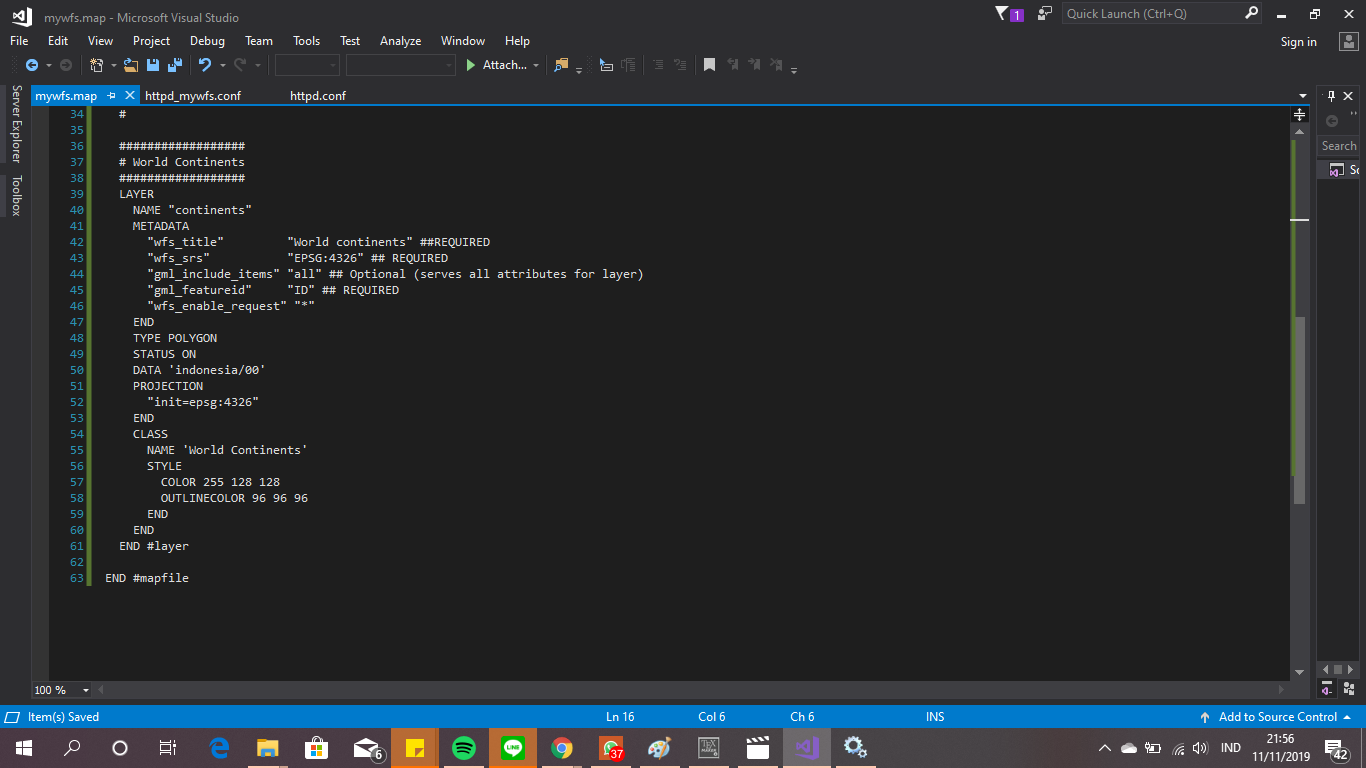
\includegraphics[width=4cm]{figures/tugas4/1174069/23.png}
  \centering
  \caption{Buka aplikasi mapproxy}
  \end{figure}
  
  \item Buka browser lalu ketikkan 127.0.0.1:8080
  \hfill\break
  \begin{figure}[H]
  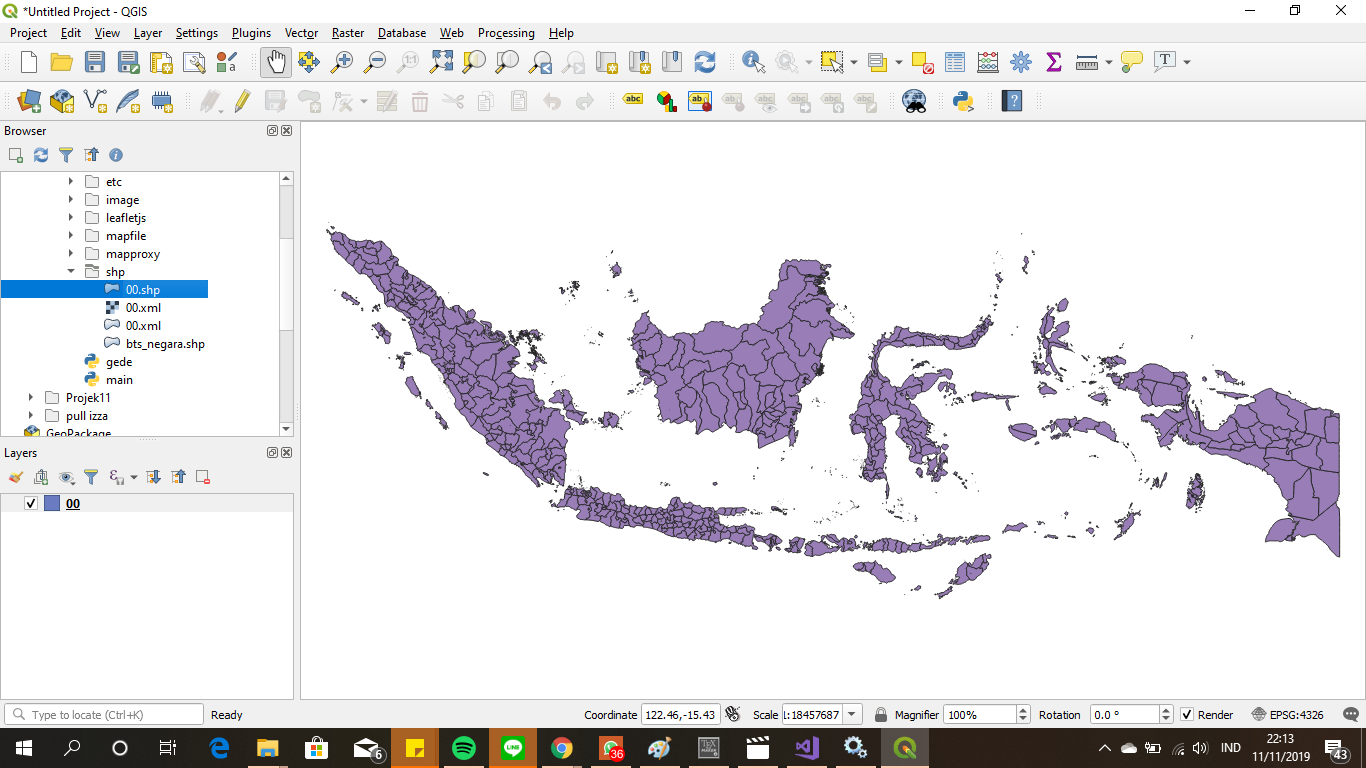
\includegraphics[width=4cm]{figures/tugas4/1174069/24.png}
  \centering
  \caption{MapProxy menampilkan map}
  \end{figure}

  \item lalu klik demo untuk melihat map
  \item lalu klik png pada agm, maka mapproxy akan menampilkan map
  \hfill\break
  \begin{figure}[H]
  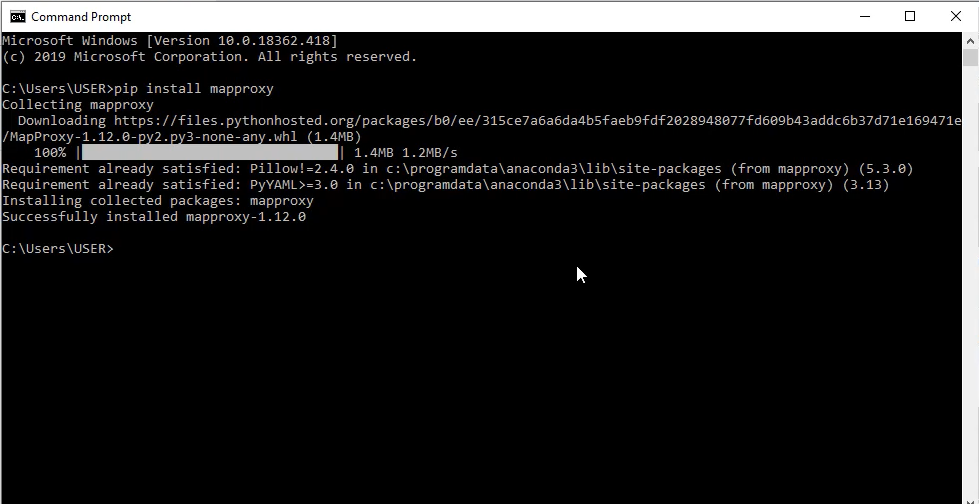
\includegraphics[width=4cm]{figures/tugas4/1174069/25.png}
  \centering
  \caption{MapProxy menampilkan map}
  \end{figure}

\end{enumerate}

\subsection{Link Youtube MapProxy dan Menjalankannya}
https://youtu.be/Y4Ru7wEsPm8